\section{Pengantar Block Cipher dan DES}

\subsection{Block Cipher}

Block cipher memecah plaintext menjadi blok-blok dengan ukuran tetap, kemudian mengenkripsi setiap blok secara independen. Berbeda dengan cipher klasik yang memproses karakter satu per satu, block cipher bekerja pada unit data yang lebih besar, memberikan keamanan dan efisiensi yang lebih baik. DES adalah contoh paling terkenal dari block cipher yang menggunakan blok 64 bit dengan kunci 56 bit efektif.

DES dikembangkan oleh IBM pada 1970-an dan distandarisasi sebagai FIPS 46 oleh NIST pada 1977 \cite{fips46_3}. Block cipher modern seperti AES menggunakan blok 128 bit dan kunci hingga 256 bit \cite{stallings2017}.

\subsection{Struktur Feistel DES}

DES menggunakan struktur Feistel dengan 16 round untuk menciptakan kebingungan yang tinggi (confusion dan diffusion). Setiap round terdiri dari empat operasi utama: Expansion, Substitution, Permutation, dan Mixing. Struktur ini dirancang untuk memastikan bahwa perubahan kecil dalam plaintext atau kunci akan menyebabkan perubahan besar dalam ciphertext, membuat analisis kriptografi menjadi sangat sulit.

Struktur Feistel memberikan confusion dan diffusion \cite{stallings2017}. Dekripsi mirip enkripsi karena operasi $F$ tidak harus invertible.

\subsection{Fungsi Round DES}

Setiap round DES menggunakan fungsi round yang sama dengan kunci subround yang berbeda. Fungsi ini menggabungkan empat operasi dasar: Expansion E, Substitution S, Permutation P, dan Mixing M. Operasi-operasi ini dirancang untuk memberikan kombinasi optimal antara keamanan dan efisiensi, dengan setiap operasi berkontribusi pada sifat confusion dan diffusion yang diinginkan.

Fungsi round DES memadukan expansion (E), S-box (S), permutation (P) \cite{fips46_3}. Kombinasi ini menciptakan avalanche effect.

\begin{figure}[htbp]
  \centering
  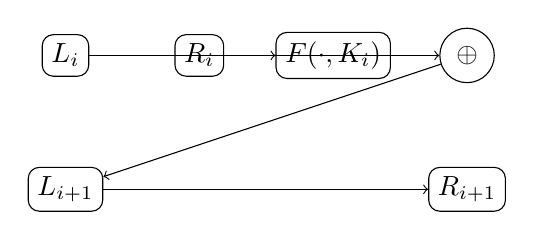
\begin{tikzpicture}[node distance=1.7cm]
    \node (l0) [draw, rounded corners] {$L_i$};
    \node (r0) [draw, rounded corners, right of=l0] {$R_i$};
    \node (f) [draw, rounded corners, right of=r0] {$F(\cdot, K_i)$};
    \node (xor) [draw, circle, right of=f] {$\oplus$};
    \node (l1) [draw, rounded corners, below of=l0] {$L_{i+1}$};
    \node (r1) [draw, rounded corners, below of=xor] {$R_{i+1}$};
    \draw[->] (l0) -- (f);
    \draw[->] (r0) -- (xor);
    \draw[->] (xor) -- (l1);
    \draw[->] (l1) -- (r1);
  \end{tikzpicture}
  \caption{Satu putaran Feistel DES.}
\end{figure}

\begin{lstlisting}[style=cstyle, caption={Satu putaran Feistel (pseudocode)}]
void des_round(uint32_t *L, uint32_t *R, uint32_t *K, uint32_t round) {
    // Expansion E: 32 bit -> 48 bit
    uint64_t expanded_R = expand_e(R[round]);
    
    // Substitution S: 48 bit -> 48 bit
    uint32_t substituted_R = substitution_s(expanded_R, K[round]);
    
    // Permutation P: 48 bit -> 48 bit
    uint32_t permuted_R = permutation_p(substituted_R);
    
    // Mixing: 48 bit -> 32 bit
    uint32_t mixed_R = mixing_m(permuted_R);
    
    // XOR dengan subkey
    R[round + 1] = mixed_R ^ K[round];
}
\end{lstlisting}

\subsection{Fungsi dan Komponen DES}

DES memiliki beberapa komponen fundamental yang bekerja sama untuk menciptakan keamanan tinggi. Initial Permutation (IP) mengacak urutan 64 bit plaintext sebelum enkripsi, sedangkan Final Permutation (FP) mengacak kembali setelah 16 round. S-box (Substitution Box) melakukan substitusi non-linear 6 bit ke 4 bit, menciptakan kebingungan yang sangat kompleks dan sulit dianalisis tanpa mengetahui desain internalnya.

\begin{table}[htbp]
  \centering
  \small
  \begin{tabular}{lll}
    \toprule
    Komponen & Fungsi & Ukuran \\
    \midrule
    Initial Permutation & Mengacak bit plaintext & 64 bit \\
    Expansion Function & Menambah 16 bit ke 48 bit & 32→48 bit \\
    S-box & Substitusi non-linear 6→4 bit & 6→4 bit (8 kotak) \\
    Permutation & Mengacak posisi bit & 32 bit \\
    Key Schedule & Menghasilkan 16 subkunci & 56→64 bit \\
    \bottomrule
  \end{tabular}
  \caption{Komponen utama DES dan fungsinya.}
\end{table}

\subsection{DES (Data Encryption Standard)}

DES distandarisasi sebagai FIPS 46 oleh NIST \cite{fips46_3}. Blok 64 bit, kunci 56 bit efektif. Kerentanan utama: brute force (56 bit) dan differential/linear cryptanalysis \cite{stallings2017}.

\subsection{Serangan terhadap DES}

DES rentan terhadap brute force (kunci 56 bit dapat dipecahkan dalam waktu wajar), differential cryptanalysis, dan linear cryptanalysis \cite{menezes1996}.

\subsection{3DES (Triple DES)}

3DES menerapkan DES tiga kali dengan kunci berbeda; keamanan efektif sekitar 112 bit \cite{stallings2017}. 3DES lebih lambat; untuk aplikasi baru gunakan AES.

\begin{table}[htbp]
  \centering
  \small
  \begin{tabular}{lcc}
    \toprule
    Metode & Keamanan & Performa \\
    \midrule
    DES & Standar, kunci pendek & Cepat \\
    3DES & Lebih aman, kunci panjang & Lebih lambat \\
    \bottomrule
  \end{tabular}
  \caption{Perbandingan DES dan 3DES.}
\end{table}

\subsection{Implementasi Praktis}

Implementasi DES hanya direkomendasikan untuk tujuan edukasi. Gunakan library teruji (OpenSSL, libsodium) untuk produksi \cite{ferguson2010}.

\begin{catatan}
Implementasi manual DES hanya direkomendasikan untuk tujuan edukasi dan pemahaman konsep. Untuk aplikasi produksi, selalu gunakan library yang telah melalui audit keamanan profesional dan validasi standar industri. Hindari implementasi sendiri dari algoritma kompleks seperti DES kecuali jika diperlukan untuk pembelajaran mendalam tentang kriptanalisis.
\end{catatan}

\subsection{Key Schedule DES}

Kunci DES 64 bit mengandung 8 bit parity, sehingga hanya 56 bit efektif. Proses key schedule:
\begin{itemize}
  \item \textbf{PC-1}: pilih 56 bit dan bagi menjadi $C_0$ dan $D_0$ (masing-masing 28 bit).
  \item \textbf{Left shift}: $C_i$ dan $D_i$ digeser 1 atau 2 bit sesuai tabel.
  \item \textbf{PC-2}: pilih 48 bit dari gabungan $C_i||D_i$ menjadi subkey $K_i$.
\end{itemize}

\begin{table}[htbp]
  \centering
  \small
  \begin{tabular}{cccccccc}
    \toprule
    Round & 1 & 2 & 3 & 4 & 5 & 6 & 7 \\
    Shift & 1 & 1 & 2 & 2 & 2 & 2 & 2 \\
    \midrule
    Round & 8 & 9 & 10 & 11 & 12 & 13 & 14 \\
    Shift & 2 & 1 & 2 & 2 & 2 & 2 & 2 \\
    \midrule
    Round & 15 & 16 & & & & & \\
    Shift & 2 & 1 & & & & & \\
    \bottomrule
  \end{tabular}
  \caption{Jadwal pergeseran kunci DES.}
\end{table}

\subsection{Serangan terhadap DES dan 3DES}

\begin{itemize}
  \item \textbf{Brute force}: 56-bit key dapat dipecahkan dengan perangkat modern.
  \item \textbf{Differential/linear cryptanalysis}: teknik analitis terhadap struktur DES.
  \item \textbf{3DES}: lebih aman tetapi lebih lambat; rentan \textit{meet-in-the-middle} dengan keamanan efektif sekitar 112 bit \cite{stallings2017}.
\end{itemize}

\subsection{Evolusi dari DES ke AES}

AES dipilih NIST (1997--2000) sebagai pemenang kompetisi; Rijndael menang \cite{fips197}. AES menggunakan blok 128 bit, kunci 128/192/256 bit.

\subsection{Pentingnya DES dalam Sejarah Kriptografi}

DES adalah cipher simetris pertama yang distandarisasi publik; konsep S-box, Feistel, confusion/diffusion tetap fundamental \cite{stallings2017}.

\begin{catatan}
Studi DES tetap penting untuk pemahaman mendalam tentang kriptografi simetris dan kriptanalisis. Banyak konsep fundamental dalam kriptografi modern, seperti confusion, diffusion, dan avalanche effect, pertama kali dipelajari secara mendalam melalui analisis DES. Meskipun tidak lagi digunakan dalam produksi, DES tetap menjadi alat edukasi yang sangat berharga.
\end{catatan}
